\chapter{Nền tảng: Các ngôn ngữ hệ thống cho phần mềm nhạy độ trễ\label{chapter:background}}
% The class prints the chapter and section titles in the running head in capitals,
% where the full title of this chapter runs into the margin.
\chaptermark{Nền tảng}

\section{Hệ thống mặt điều khiển RAN và gNB-CU-CP}\label{sec:ranarch}
Kiến trúc NG-RAN tách gNB thành đơn vị trung tâm (gNB-CU) và các đơn vị phân tán, với mặt
điều khiển (gNB-CU-CP) xử lý RRC và quản lý kết nối cho mỗi
UE~\cite{3gpp38401,3gpp38300,3gpp38331}. Hệ thống mặt điều khiển như vậy phải đáp ứng yêu cầu
phi chức năng khắt khe: tốc độ sự kiện rất cao (di động UE, cơn bão báo hiệu), giới hạn độ trễ
nghiêm ngặt và dự đoán được mà đặc tả dịch vụ và RAN 5G lượng hoá thành
KPI~\cite{3gpp38913,3gpp22261}, phần mềm sống lâu với độ phức tạp liên tục tiến hoá, và khối
lượng tương tranh cao. Trong các hệ thống này hành vi trường hợp xấu nhất và đuôi, thay vì
trung bình, quyết định liệu hạn chót được đáp ứng, điều thúc đẩy trọng tâm khả năng dự đoán
của luận văn này.

Về chức năng, gNB được tách rời theo hai trục độc lập. Trục thứ nhất là tách
\emph{trung tâm/phân tán}: đơn vị trung tâm (gNB-CU) lưu các tầng cao hơn của ngăn xếp giao
thức, trong khi một hoặc nhiều đơn vị phân tán (gNB-DU) lưu các tầng thấp hơn, nhạy thời gian
hơn, gần vô tuyến. Trục thứ hai là tách \emph{mặt điều khiển/mặt người dùng} bên trong đơn vị
trung tâm, tách chức năng mặt điều khiển (gNB-CU-CP) khỏi chức năng mặt người dùng (gNB-CU-UP).
Các phần này giao tiếp qua giao diện chuẩn hoá: NG về lõi 5G, F1 giữa CU và DU, và E1 giữa
CU-CP và CU-UP~\cite{3gpp38401,3gpp38300,3gpp38463}. Sáng kiến Open-RAN chuẩn hoá thêm các
giao diện này để mỗi phần có thể do nhà cung cấp khác cung cấp và chạy như phần mềm trên phần
cứng thương mại~\cite{polese2023oran}. Hình~\ref{fig:ngran} đặt phân hệ nghiên cứu trong luận
văn này, Quản lý Ngữ cảnh UE (UECM), bên trong gNB-CU-CP: nó sở hữu trạng thái mặt điều khiển
theo từng UE và điều phối báo hiệu RRC cùng thủ tục di động, nên tính đúng đắn và hành vi
thời gian của nó đại diện cho mặt điều khiển nói chung.

\begin{figure}[ht]
\centering
\begin{tikzpicture}[
    font=\small, >={Stealth[length=2.4mm]},
    box/.style={draw, rounded corners, minimum height=1.0cm, minimum width=1.7cm,
                align=center, fill=gray!8},
    cpbox/.style={draw, rounded corners, align=center, fill=blue!8},
    upbox/.style={draw, rounded corners, minimum width=3.1cm, minimum height=0.8cm,
                  align=center, fill=green!8},
    uecm/.style={draw, rounded corners, minimum width=2.7cm, minimum height=0.62cm,
                 fill=red!14, align=center}
  ]
  \node[box] (ue) at (0,0)   {UE};
  \node[box] (du) at (2.4,0) {gNB-DU};

  % Control plane, with UE Context Management shown nested inside it
  \node[font=\footnotesize\bfseries] (cpttl) at (7.2,1.7) {gNB-CU-CP};
  \node[uecm] (uecm) at (7.2,0.85) {UE Context\\ Management};
  \begin{scope}[on background layer]
    \node[cpbox, fit=(cpttl)(uecm), inner sep=6pt] (cp) {};
  \end{scope}
  % User plane
  \node[upbox] (up) at (7.2,-0.95) {gNB-CU-UP};

  \begin{scope}[on background layer]
    \node[draw, dashed, rounded corners, fill=gray!3,
          fit=(cp)(up), inner sep=10pt, label={[font=\footnotesize\bfseries]above:gNB-CU}] (cu) {};
  \end{scope}

  \node[box] (core) at (11.4,0) {5GC};

  \draw[<->] (ue) -- node[above,font=\scriptsize]{Uu} (du);
  \draw[<->] (du.east)         -- node[above,font=\scriptsize]{F1} (cu.west |- du);
  \draw[<->] (cu.east |- core) -- node[above,font=\scriptsize]{NG} (core.west);
  \draw[<->] (cp.south) -- node[right,font=\scriptsize]{E1} (up.north);
\end{tikzpicture}
\caption[Vị trí phân hệ nghiên cứu trong NG-RAN 5G]{Vị trí phân hệ nghiên cứu trong NG-RAN 5G. gNB được tách thành đơn vị
phân tán (gNB-DU) và đơn vị trung tâm (gNB-CU), và đơn vị trung tâm lại được tách thành chức
năng mặt điều khiển (gNB-CU-CP) và mặt người dùng (gNB-CU-UP), nối qua các giao diện chuẩn
F1, E1 và NG. Quản lý Ngữ cảnh UE (được tô) là trình quản lý trạng thái mặt điều khiển theo
từng UE bên trong gNB-CU-CP mà luận văn này tái hiện thực và đo
lường.\label{fig:ngran}}
\end{figure}

\section{Độ trễ, thông lượng và khả năng dự đoán trong phần mềm thời gian thực}\label{sec:predictability}
\sectionmark{Độ trễ và khả năng dự đoán}
Hệ thống nhạy độ trễ được đánh giá ít hơn bằng lượng công việc trung bình mà bằng mức độ
\emph{dự đoán được} khi thực hiện. Ba chỉ số phải được phân biệt. \emph{Thông lượng} là tốc
độ bền vững của thao tác hoàn thành, \emph{độ trễ} là thời gian một thao tác riêng lẻ mất, và
\emph{jitter} là độ biến thiên của độ trễ đó. Một hệ thống có thể có độ trễ trung bình xuất
sắc và vẫn thường xuyên trễ hạn. Các con số có ý nghĩa do đó là độ trễ \emph{đuôi} phân vị
cao, phân vị thứ 99 (p99) và 99.9 (p99.9), thay vì trung bình. Ở quy mô mạng, độ trễ đuôi chi
phối hành vi người dùng thấy được: khi một hành động của người dùng lan ra nhiều thao tác nội
bộ, thao tác chậm nhất quyết định thời gian phản hồi, nên trễ hiếm trên mỗi thao tác trở thành
trễ thường gặp trên mỗi yêu cầu~\cite{dean2013tail}. Phần mềm trung tâm dữ liệu và mạng hiện
đại ngày càng vận hành trong chế độ mà độ trễ liên quan đo bằng micro giây, dải mà chi phí
hệ điều hành và phần mềm thông thường không còn không đáng
kể~\cite{barroso2017microseconds}. Nghiên cứu đo chi tiết cho thấy, ngay cả ở mức sử dụng vừa
phải, hiệu ứng phần cứng, hệ điều hành và ứng dụng như nhiễu nền, lập lịch, định tuyến ngắt
và trạng thái tiết kiệm năng lượng phồng đuôi xa vượt xa dự đoán của mô hình hàng
đợi~\cite{li2014tales}. Hình~\ref{fig:tailconcept} đặt hai hiệu ứng cạnh nhau: khoảng cách giữa
trung vị và các phân vị cao, và hiệu ứng lan truyền biến trễ hiếm trên mỗi thao tác thành trễ
thường gặp trên mỗi thủ tục.

\begin{figure}[ht]
\centering
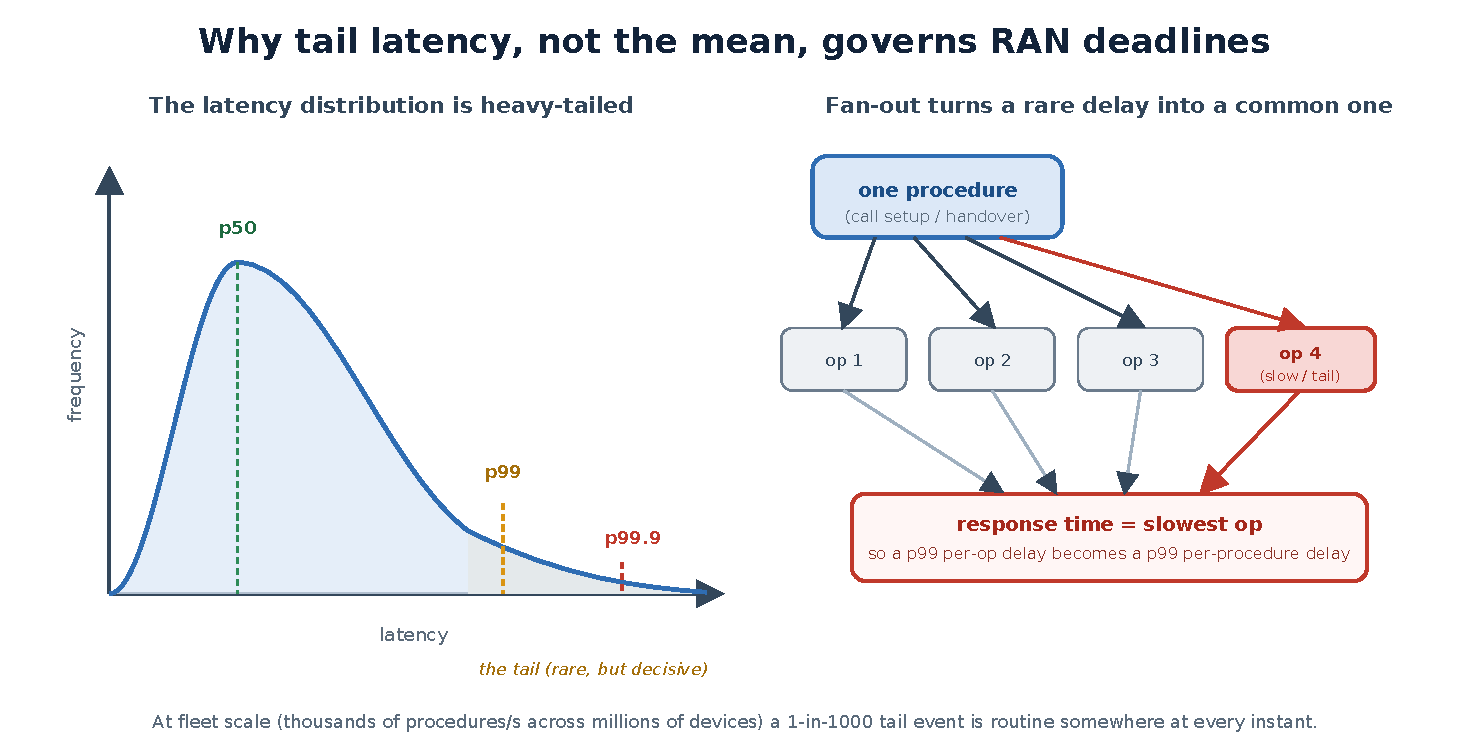
\includegraphics[width=0.78\linewidth]{diagrams/pdf/11_tail_latency_concept.pdf}
\caption[Vì sao đuôi, không phải trung bình, quyết định hạn chót RAN]{Vì sao đuôi, không phải trung bình, quyết định hạn chót RAN. Bên trái, hầu hết thao tác
kết thúc nhanh và một số ít lâu hơn nhiều, nên p99 và p99.9 nằm xa bên phải trung vị. Bên
phải, một thủ tục như thiết lập cuộc gọi chạy nhiều thao tác và chỉ kết thúc khi thao tác
chậm nhất xong, nên trễ chạm một thao tác trong một trăm lần chạm tới phần lớn hơn nhiều của
các thủ tục. Ở quy mô đội tàu, trễ một trong nghìn lần đang xảy ra ở đâu đó mọi
khoảnh khắc.\label{fig:tailconcept}}
\end{figure}

Hệ thống thời gian thực thường được phân cấp theo hệ quả của việc trễ hạn: trong thời gian
thực \emph{cứng} một lần trễ là thất bại, trong thời gian thực \emph{firm} kết quả muộn vô
dụng nhưng không thảm hoạ, và trong thời gian thực \emph{mềm} một lần trễ chỉ làm giảm chất
lượng. Mặt điều khiển RAN nên được xem là thời gian thực mềm đến firm: một phản hồi báo hiệu
trễ thỉnh thoảng làm giảm dịch vụ chứ không gây nguy hiểm, nhưng ở quy mô đội tàu và dưới cơn
bão báo hiệu các suy giảm đó tích lũy thành vấn đề tin cậy toàn mạng. Điều này càng nặng bởi
hành vi hàng đợi: khi tải đưa vào tiến gần công suất phục vụ, trễ hàng đợi tăng mạnh và đuôi
độ trễ bùng nổ gần bão hoà. Mô tả hệ thống do đó cần đẩy tải không chỉ ở mức danh nghĩa mà
\emph{vào quá tải}, đó là lý do phần đánh giá trong luận văn này quét tải lên và vượt điểm
bão hoà.

Đo độ trễ đuôi đúng bản thân nó là cạm bẫy. Một bộ sinh tải vòng kín ngây thơ chờ mỗi phản hồi
trước khi phát yêu cầu tiếp theo mắc \emph{coordinated omission}: khi hệ thống đứng, bộ sinh
cũng đứng theo và đơn giản không ghi các yêu cầu lẽ ra đã tới trong lúc đứng, che có hệ thống
chính xác cái đuôi mà nó phải lộ ra. Hình~\ref{fig:coord} đối chiếu hai mô hình bộ sinh.
Phân biệt bên dưới là mô hình hoá, không phải chi tiết hiện thực. Trong hệ kín một yêu cầu mới
chỉ kích hoạt khi yêu cầu trước hoàn thành, trong khi hệ mở các lần đến độc lập với hoàn thành,
và hai mô hình cho hành vi thời gian phản hồi khác hệ thống trên cùng quy trình phục vụ, với
mô hình kín báo cáo con số thấp hơn~\cite{schroeder2006openclosed}. Đo lường đúng do đó cần mô
hình vòng mở với lịch dự định, hiệu chỉnh coordinated omission, histogram độ trễ độ phân giải
cao giữ độ chi tiết qua nhiều bậc độ lớn, và báo cáo thống kê chặt với lần chạy lặp và khoảng
tin cậy thay vì ước lượng điểm
đơn~\cite{georges2007rigorous}. Các kỹ thuật này được áp dụng ở
Chương~\ref{chapter:eval}.

\begin{figure}[ht]
\centering
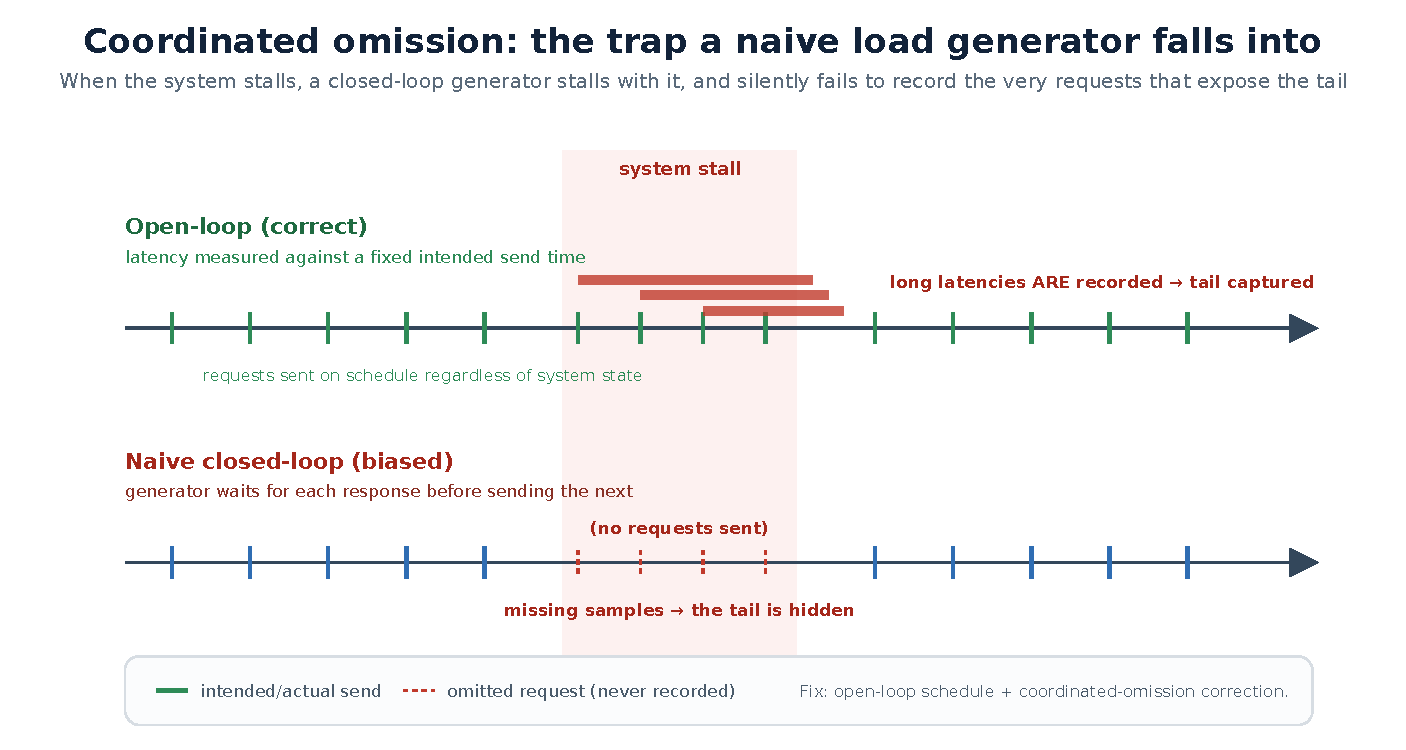
\includegraphics[width=0.78\linewidth]{diagrams/pdf/16_coordinated_omission.pdf}
\caption[Coordinated omission dưới tải vòng mở và vòng kín]{Coordinated omission. Bộ sinh vòng mở phía trên gửi theo lịch cố định ngay cả khi hệ thống
đứng, và tính thời gian mỗi yêu cầu từ lúc đến hạn, nên yêu cầu bị kẹt được ghi với toàn bộ
trễ và đuôi hiện ra. Bộ sinh vòng kín phía dưới chỉ gửi yêu cầu tiếp theo sau khi phản hồi
trước tới. Khi hệ thống đứng nó cũng ngừng gửi, nên các yêu cầu chậm nhất không bao giờ được
phát và không bao giờ được đo, và đuôi biến mất khỏi dữ
liệu.\label{fig:coord}}
\end{figure}

\section{C++ cho hệ thống nhạy độ trễ}\label{sec:cpplatency}
C++ là ngôn ngữ mặc định cho phần mềm mặt điều khiển RAN vì lý do chính đáng. Nó mang trừu
tượng không chi phí, kiểm soát trực tiếp bố cục và cấp phát bộ nhớ, hủy xác định qua idiom
Resource Acquisition Is Initialization (RAII), và trình biên dịch, thư viện cùng công cụ phân
tích trưởng thành, tất cả không có bộ thu gom rác có thể chèn khoảng dừng khó đoán. C++ hiện
đại (C++11 trở đi) thêm con trỏ thông minh (\texttt{std::unique\_ptr}, \texttt{std::shared\_ptr})
tự động hoá sở hữu, ngữ nghĩa move tránh sao chép thừa, và mô hình bộ nhớ chính thức với
\texttt{std::atomic} cho tương tranh có khóa và không khóa. Các tính năng này cho phép viết mã
hệ thống nhanh và, với kỷ luật, tương đối an toàn.

Khó khăn là trình biên dịch không thực thi an toàn này. Lập trình viên mới thực thi. RAII và
con trỏ thông minh giảm lỗi vòng đời mà không loại bỏ hết. Con trỏ hoặc tham chiếu thô có thể
sống lâu hơn đối tượng trỏ tới, biến đổi container có thể vô hiệu iterator, đối tượng có thể
bị dùng sau khi đã move, và không gì trong hệ kiểu ngăn đối tượng mutable được chia sẻ và ghi
bởi nhiều luồng cùng lúc. Kết quả là danh mục lỗi quen thuộc, use-after-free, double-free, tràn
bộ đệm, tranh chấp dữ liệu, deadlock và vô hiệu iterator, dễ đưa vào và tốn kém để tìm ở quy
mô viễn thông. Lỗi hỏng bộ nhớ loại này là vấn đề bảo mật dai dẳng hàng thập kỷ, và các giảm
thiểu triển khai vẫn chỉ là phòng thủ một
phần~\cite{szekeres2013sok}. Mức độ phổ biến được ghi nhận rõ trong công nghiệp. Vấn đề an toàn
bộ nhớ chiếm khoảng 70\,\% lỗ hổng bảo mật Microsoft
báo cáo~\cite{msrc2019memory}, và Google báo cáo giảm mạnh lỗ hổng loại này khi ngôn ngữ an
toàn bộ nhớ được áp dụng trên Android, xuống dưới một phần năm tổng lỗ hổng nền tảng đó vào
năm 2025~\cite{google2022android,vanderstoep2025android}. Danh mục cụ thể này được phát triển
chi tiết ở Chương~\ref{chapter:context} và là cơ sở cho nghiên cứu tiêm lỗi ở
Chương~\ref{chapter:eval}.

Thực hành C++ giảm thiểu các lỗi này bằng công cụ thay vì đảm bảo ngôn ngữ, và công cụ vốn
dĩ chỉ một phần. Bộ dò lỗi động như AddressSanitizer (ASan), ThreadSanitizer (TSan) và
UndefinedBehaviorSanitizer phát hiện nhiều lỗi, nhưng chỉ trên đường mã mà kiểm thử cụ thể
thực sự chạy với đầu vào đúng, và chúng đặt chi phí chạy và bộ nhớ khiến chúng không phù hợp
sản xuất. TSan đặc biệt chỉ báo cáo tranh chấp dữ liệu xảy ra trong một lần chạy, nên tranh
chấp chỉ lộ dưới xen kẽ hiếm có thể lọt. Bộ phát hiện deadlock của nó thừa hưởng giới hạn đó
từ kỹ thuật nó hiện thực, suy luận tiềm năng deadlock từ đồ thị khóa của một trace
đơn~\cite{bensalem2005deadlock}, và nó được phát hành như thành phần thử nghiệm chỉ bao họ
mutex POSIX~\cite{tsandeadlock}. Phân tích tĩnh giúp nhưng mắc false negative và không lý
giải toàn chương trình. Phát hiện do đó là nỗ lực tốt nhất và sau sự kiện, đúng tình huống mà
ngôn ngữ có đảm bảo lúc biên dịch nhằm thay đổi.

Điều đó mô tả C++ như có thể triển khai hôm nay, và ngôn ngữ không đứng yên. Từ năm 2023 ủy
ban tiêu chuẩn theo đuổi \emph{profiles}: tập quy tắc đặt tên bao phủ an toàn kiểu, biên, vòng
đời và số học mà triển khai tuân thủ phải thực thi ở mọi nơi được
bật~\cite{sutter2025profiles}. Hướng đó được chọn thay vì \emph{Safe C++}, đề xuất tập con an
toàn với kiểm tra mượn và thư viện chuẩn riêng, tức mô hình Rust diễn đạt trong
C++~\cite{baxter2024safecpp}. Phép so sánh ở đây vẫn giữ hiệu lực. Profiles chưa được chuẩn
hoá, và tháng 1 năm 2026 chính tác giả vẫn kêu gọi hiện thực và coi thiết kế các profile ban
đầu là việc còn phải
làm~\cite{vandevoorde2026profiles}. Profile tương tranh, cái liên quan các lớp lỗi được liệt kê
ở Chương~\ref{chapter:context}, được đặt sau tập ban đầu và không nằm trong đó: ``cần định
nghĩa và hiện thực thêm profile, đặc biệt một profile
tương tranh''~\cite{vandevoorde2026profiles}. Quy tắc chỉ thực thi khi bật cũng là thứ khác
với thuộc tính hệ kiểu mang vô điều kiện, nhất là khi thực thi là kiểm tra chạy chứ không phải
từ chối biên dịch. Các bản hiện thực so sánh ở đây do đó được xây theo C++23 như đã đặc tả và
phát hành, và Mục~\ref{sec:threats} ghi điều đó ghim phép so sánh vào đâu.

\section{Mô hình sở hữu và an toàn của Rust}
Rust thực thi an toàn bộ nhớ và không tranh chấp dữ liệu lúc biên dịch qua mô hình sở hữu và
mượn~\cite{klabnik2023rust}, và đi kèm công cụ hiện đại trong Cargo cùng kiểm thử tích hợp. Hệ
kiểu cấm tĩnh biến đổi trạng thái chia sẻ và giam các ngoại lệ không tránh khỏi vào mã
\texttt{unsafe} giữ sau API an toàn~\cite{jung2021safe}.

Các đảm bảo này dựa trên hơn khẳng định. Tính đúng đắn của mảnh an toàn của ngôn ngữ, gồm vai
trò \texttt{unsafe} như lối thoát được đánh dấu rõ, đã được thiết lập chính thức bởi dự án
RustBelt~\cite{jung2018rustbelt}, và kỷ luật alias mà ngay cả mã \texttt{unsafe} phải tuân theo
đã được cho ngữ nghĩa vận hành
chính xác~\cite{jung2020stacked}. Bằng chứng thực nghiệm ủng hộ mô hình trong thực tế: trong
mã nguồn thật \texttt{unsafe} được dùng tiết kiệm và cục
bộ~\cite{qin2020rust,astrauskas2020unsafe}, và nghiên cứu mọi CVE an toàn bộ nhớ Rust tìm thấy
mỗi CVE trừ một lỗi trình biên dịch đều liên quan mã
\texttt{unsafe}~\cite{xu2021rustcve}. Lưu ý là không an toàn lan qua phụ thuộc. Ít hơn một phần
ba thư viện dùng \texttt{unsafe} trực tiếp, nhưng phần lớn hơn nhiều không thể kiểm tra tĩnh
đầy đủ vì nó ẩn đâu đó trong chuỗi
gọi~\cite{evans2020rust}, đó là lập luận thêm để giữ lõi an toàn quan trọng của phân hệ không
cần \texttt{unsafe}, như luận văn này làm.

Một thuộc tính quan trọng nhất trong bối cảnh nhạy độ trễ. An toàn này đến từ hệ kiểu và bộ
kiểm tra mượn, không từ công cụ chạy, và được dự định là \emph{không chi phí}. Nghiên cứu hệ
thống lập luận Rust đạt an toàn không chi phí thu gom rác hay kiểm tra chạy, và còn cho phép
kỹ thuật hiệu quả khó trong
C~\cite{balasubramanian2017rust}. Liệu tuyên bố không chi phí có đúng với khối lượng mặt điều
khiển viễn thông chính là thuộc tính mà luận văn này đánh giá.

Cụ thể, bộ kiểm tra mượn từ chối lúc biên dịch chính use-after-free phác thảo ở phần giới
thiệu: chương trình giải phóng ngữ cảnh trong khi tham chiếu tới nó vẫn còn sống thì không
build. Hình~\ref{fig:borrowuaf} đặt lỗi đó ở dạng Quản lý Ngữ cảnh UE cạnh bản C++, biên dịch
và chỉ bị bắt, nếu có, lúc chạy.

\begin{figure}[ht]
\centering
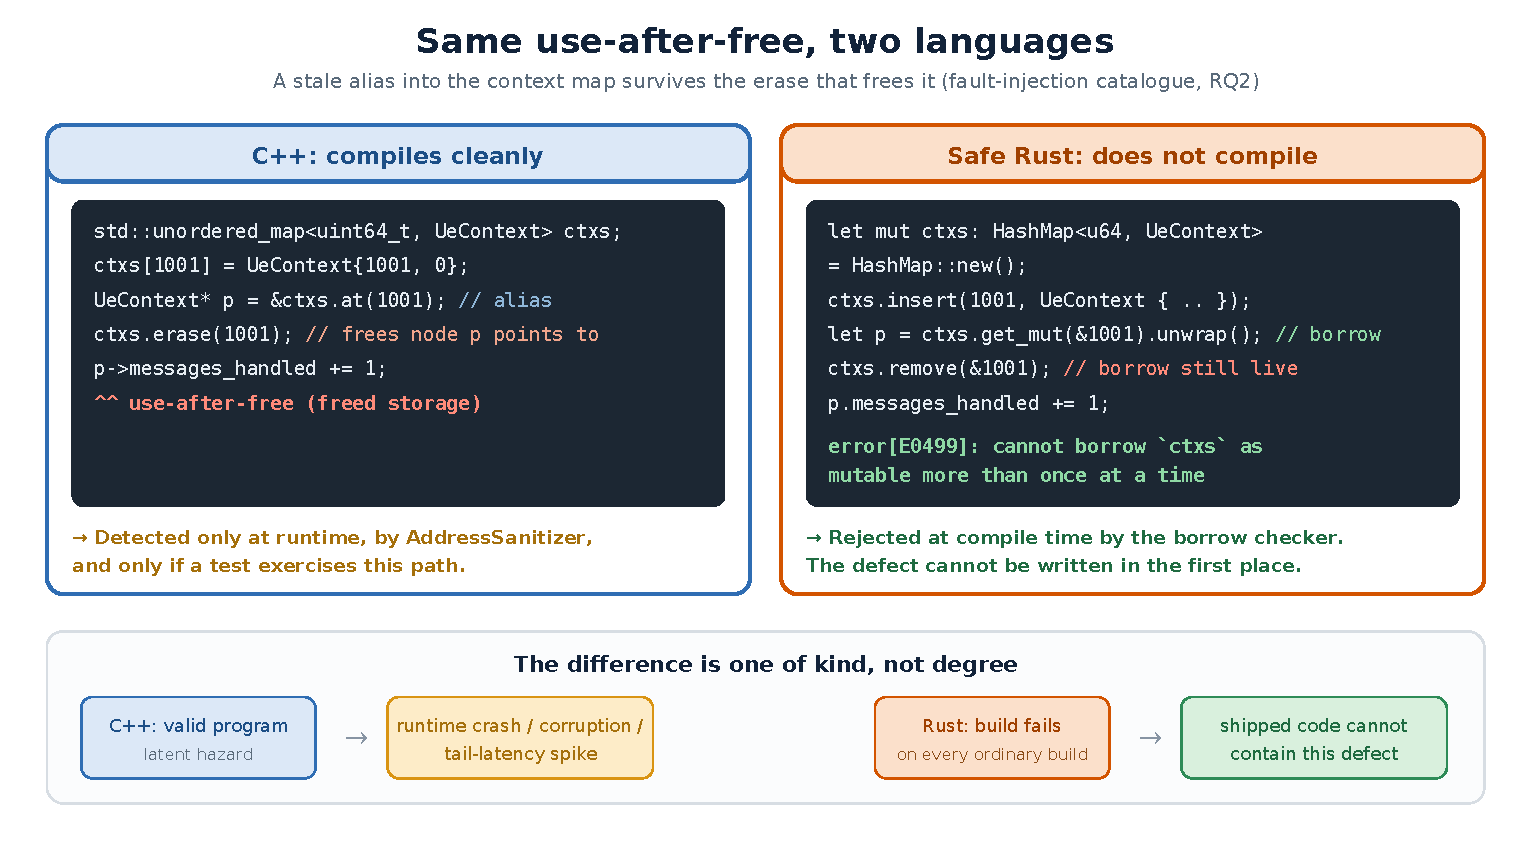
\includegraphics[width=0.78\linewidth]{diagrams/pdf/08_borrow_checker_uaf.pdf}
\caption[Cùng use-after-free trong C++ và Rust an toàn]{Cùng lỗi use-after-free trong C++ và Rust an toàn. Alias cũ vào bản đồ ngữ cảnh sống
sót sau \texttt{erase}/\texttt{remove} giải phóng nó: trong C++ mã này biên dịch và chỉ bị
bắt lúc chạy (và chỉ dưới AddressSanitizer, trên đường mà kiểm thử chạy), trong khi Rust an
toàn bộ kiểm tra mượn từ chối lúc biên dịch (\texttt{E0499}), nên lỗi không thể viết ra. Khác
biệt là về loại, không phải mức độ.\label{fig:borrowuaf}}
\end{figure}

Cùng kỷ luật mở rộng sang tương tranh. Rust mã hoá an toàn luồng trong hệ kiểu qua marker trait
\texttt{Send} và \texttt{Sync}: giá trị chỉ qua ranh giới luồng nếu kiểu là \texttt{Send}, và
chỉ chia sẻ bằng tham chiếu qua luồng nếu là \texttt{Sync}. Chia sẻ giá trị cho phép biến đổi
không đồng bộ do đó là lỗi biên dịch, không phải tranh chấp tiềm ẩn. Đây là thuộc tính Rust
quảng bá là ``fearless concurrency.'' Xử lý lỗi cũng tường minh: thao tác có thể thất bại trả
về giá trị \texttt{Result} mà người gọi phải xử lý, thay vì ném ngoại lệ làm unwind qua luồng
điều khiển ẩn. Cả chi phí lẫn luồng điều khiển của đường thất bại do đó vẫn nhìn thấy được,
đó là lợi thế trong mã nhạy độ trễ nơi bất ngờ ở đuôi mới quan trọng.

Rust không phải ngôn ngữ an toàn bộ nhớ duy nhất, và lý do phép so sánh ở đây vẽ với C++ thay
vì với runtime có quản lý thuộc cùng mô hình này. Java, C\# và Go đạt an toàn bộ nhớ qua runtime
và thu gom rác, đánh đổi xuất sắc cho nhiều phần mềm và kém cho mặt điều khiển nhạy độ trễ đuôi:
khoảng dừng thu gom là nguồn độ trễ đuôi được công nhận trong hệ thống
lớn~\cite{dean2013tail}, và runtime có quản lý từ bỏ kiểm soát bố cục bộ nhớ và lập lịch mà
miền này dựa vào. C, ở cực kia, không an toàn bộ nhớ như C++ trong khi ít trừu tượng hơn để
xây hệ thống lớn. Rust là ngôn ngữ được hỗ trợ rộng đầu tiên kết hợp an toàn bộ nhớ và luồng
lúc biên dịch với không có bộ thu gom rác và thông lượng cùng bộ nhớ cạnh C và
C++~\cite{balasubramanian2017rust,jung2021safe,bugden2022rust}. Đó là lý do ngôn ngữ có quản lý
nằm ngoài phạm vi và lý do phép so sánh có ý nghĩa cho phần mềm mặt điều khiển RAN là C++ với
Rust.

Bảng~\ref{tab:langmodel} đặt cơ chế hai ngôn ngữ cạnh nhau. Phân biệt nó xây quanh không phải
mối nguy mỗi ngôn ngữ gọi tên gì, vì cả hai gọi tên gần giống nhau, mà \emph{khi nào} và \emph{bởi
cái gì} mỗi thứ bị loại trừ, và hai hàng cuối đánh dấu nơi câu trả lời không còn là ``bởi
trình biên dịch'' với cả hai.

\begin{table}[H]
\centering
\small
\caption[Cách mỗi ngôn ngữ thực thi các thuộc tính được đo]{Cách mỗi ngôn ngữ thực thi các thuộc tính mà luận văn này đo. Các hàng trên quy
tắc là nơi hai ngôn ngữ khác về loại chứ không chỉ mức độ: trình biên dịch từ chối chương trình
loại trừ lỗi khỏi mọi lần thực thi, trong khi bộ dò lỗi chỉ loại trừ khỏi các lần thực thi mà
kiểm thử có công cụ tình cờ chạy. Các hàng dưới quy tắc là ranh giới phát triển ở
Chương~\ref{chapter:context} và đo ở Chương~\ref{chapter:eval}, nơi không ngôn ngữ nào có đảm
bảo tĩnh.\label{tab:langmodel}}
\renewcommand{\arraystretch}{1.2}
\begin{tabular}{@{}R{0.20\linewidth} R{0.36\linewidth} R{0.36\linewidth}@{}}
\hline\hline
Khía cạnh & C++ hiện đại & Rust \\
\hline
Vòng đời đối tượng & RAII và con trỏ thông minh, áp dụng theo quy ước. Con trỏ hoặc tham chiếu thô có thể sống lâu hơn đối tượng trỏ tới & Sở hữu: mỗi giá trị có một chủ sở hữu và bị giải phóng đúng một lần \\
Alias & Không hạn chế: bất kỳ số alias mutable nào cũng có thể cùng tồn tại & Mượn: hoặc một tham chiếu mutable hoặc nhiều tham chiếu chia sẻ, không bao giờ cả hai \\
Biên & Không kiểm tra trên \texttt{operator[]}, chỉ kiểm tra qua \texttt{at()} & Kiểm tra mặc định, bỏ qua nơi chỉ số chứng minh được trong phạm vi \\
An toàn luồng & Không diễn đạt trong hệ kiểu: chia sẻ đối tượng mutable qua luồng vẫn biên dịch & Marker trait \texttt{Send} và \texttt{Sync}. Chia sẻ không đồng bộ là lỗi kiểu \\
Báo hiệu lỗi & Ngoại lệ hoặc mã lỗi: đường thất bại có thể vô hình tại điểm gọi & Giá trị \texttt{Result} người gọi phải xử lý. Đường thất bại tường minh \\
Lối thoát & Toàn bộ ngôn ngữ & Khối \texttt{unsafe}, có giới hạn và đếm được cơ học \\
Giai đoạn phát hiện & Chạy, dưới bộ dò lỗi đúng, trên đường kiểm thử chạy & Biên dịch, trên mọi build thường, bất kể độ phủ kiểm thử \\
\hline
Thứ tự khóa & Không kiểm tra & Không kiểm tra \\
Tính nguyên tử của thao tác ghép & Không kiểm tra & Không kiểm tra \\
\hline
\end{tabular}
\end{table}

\section{Mô hình tương tranh cho phần mềm mặt điều khiển}
Cách cấu trúc tương tranh định hình cả tính đúng đắn lẫn độ trễ đuôi. Mô hình chi phối là
tương tranh \emph{bộ nhớ chia sẻ}, trong đó luồng biến đổi trạng thái chung được bảo vệ bởi
mutex và atomic. Nó linh hoạt, nhưng là nguồn tranh chấp, deadlock, tranh chấp khóa và đảo
ngược ưu tiên, và trường hợp xấu nhất khó giới hạn. Phương án thay thế là tương tranh
\emph{truyền thông} hoặc \emph{không chia sẻ}, trong đó trạng thái được phân vùng để mỗi phần
do một luồng sở hữu và mọi tương tác qua thông điệp, như mô hình actor. Nó đổi linh hoạt lấy
khả năng mở rộng và lý luận đơn giản hơn nhiều, và ánh xạ tự nhiên lên phân vùng theo UE, vì
trạng thái mỗi UE phần lớn độc lập. Lựa chọn cũng dịch chuyển đại lượng đo ở đây: cấu trúc
một luồng mỗi lõi tự thay đổi độ trễ đuôi ứng
dụng~\cite{enberg2019threadpercore}, nên mô hình được giữ cố định giữa hai bản hiện thực thay
vì giao cho idiom mỗi ngôn ngữ. Hình~\ref{fig:concmodels} đối chiếu hai mô hình.

\begin{figure}[ht]
\centering
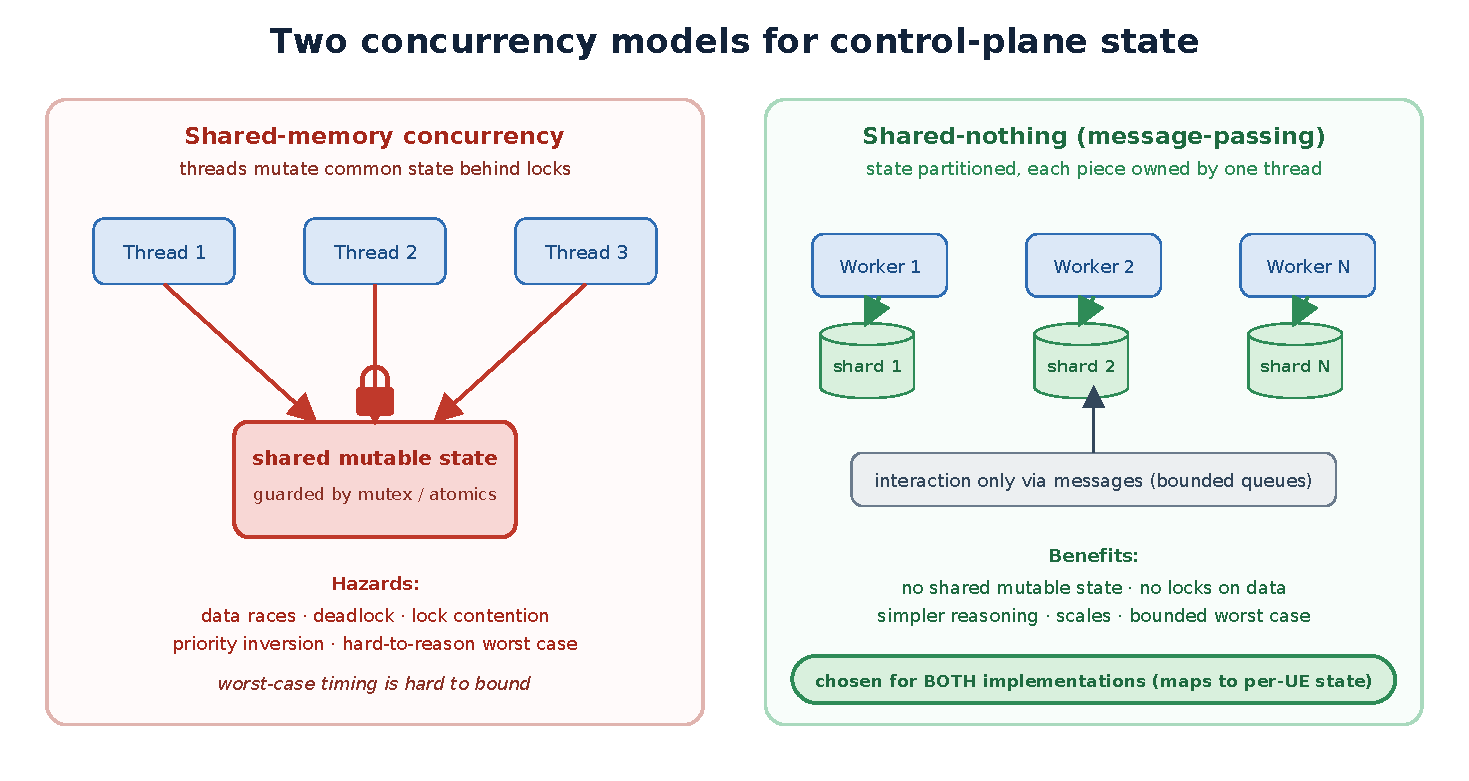
\includegraphics[width=0.78\linewidth]{diagrams/pdf/12_concurrency_models.pdf}
\caption[Hai mô hình tương tranh cho trạng thái mặt điều khiển]{Hai mô hình tương tranh cho trạng thái mặt điều khiển. Tương tranh bộ nhớ chia sẻ (trái)
cho luồng biến đổi trạng thái chung sau khóa và là nguồn tranh chấp dữ liệu, deadlock và tranh
chấp khóa, với trường hợp xấu nhất khó giới hạn. Truyền thông không chia sẻ (phải) phân vùng
trạng thái để mỗi shard do một worker sở hữu và mọi tương tác qua hàng đợi có giới hạn, loại
khóa trên dữ liệu ngữ cảnh và ánh xạ lên phân vùng theo UE. Đây là mô hình hai bản hiện thực
áp dụng.\label{fig:concmodels}}
\end{figure}

Cấu trúc thứ ba, runtime bất đồng bộ trên bộ lập lịch work-stealing, là idiom trong cả hai
ngôn ngữ và không được dùng trong cả hai. Hành vi thời gian của nó thuộc runtime, không thuộc
ngôn ngữ chứa nó: nghiên cứu thời gian thực về Rust bất đồng bộ tìm một ứng dụng đáp ứng hoặc
trễ hạn tùy runtime và ánh xạ ưu tiên luồng, và cấu hình đáp ứng hạn không phải cấu hình
work-stealing
thông thường~\cite{skoudlil2025asyncrust}. Áp dụng runtime như vậy sẽ nhập biến thiên mà nghiên
cứu này tồn tại để loại trừ, và Mục~\ref{sec:relatedwork} quay lại phép so sánh mà nó không bị
loại trừ.

Hàng đợi giữa nhà sản xuất và người tiêu thụ là lựa chọn thứ hai, độc lập. Hàng đợi không giới
hạn che quá tải và để độ trễ cùng bộ nhớ tăng không giới hạn. Hàng đợi \emph{có giới hạn}, dù
chặn để backpressure hay loại bỏ, giới hạn bộ nhớ trường hợp xấu nhất và làm quá tải nhìn thấy
được, điều độ trễ đuôi dự đoán được đòi hỏi. Cả hai lựa chọn cố định kiến trúc mà hai bản hiện
thực dùng ở Chương~\ref{chapter:design}: thiết kế không chia sẻ, một luồng mỗi shard, trong đó
trạng thái UE chia thành các lát độc lập gọi là \emph{shard}, mỗi lát do đúng một luồng worker
sở hữu, nên không hai luồng chạm cùng ngữ cảnh. Yêu cầu tới shard qua hàng đợi đa nhà sản xuất,
một người tiêu thụ có giới hạn chặn khi đầy.

\section{Khả năng tương tác giữa C++ và Rust}\label{sec:interop}
Áp dụng ngôn ngữ mới trong hệ thống lớn sẵn có buộc phải tăng dần: thành phần Rust phải cùng
tồn tại và được gọi từ mã nguồn C++ đáng kể. Mẫu số chung cho việc đó là giao diện nhị phân
ứng dụng C (ABI). Rust có thể lộ hàm với liên kết \texttt{extern "C"} và đưa ra \emph{handle
mờ} tới đối tượng do Rust sở hữu, mà C++ gọi qua header C. Công cụ tự động hoá một phần:
\texttt{bindgen} (binding Rust từ header C), \texttt{cbindgen} (header C từ Rust), và crate
\texttt{cxx} (cầu hai chiều an toàn hơn). Tương tác không miễn phí. Vượt ranh giới bước ra ngoài
ngôn ngữ được kiểm tra, nên đường ghép phải chứa mã \texttt{unsafe}, giá trị phức tạp hơn đơn
giản nhất cần marshalling, và giao diện ngoại phải được thiết kế có chủ đích. Kích thước đường
ghép, \texttt{unsafe} nó tập trung, và chi phí vượt ranh giới mỗi lần gọi là đại lượng RQ4 đo
ở Chương~\ref{chapter:eval}.

Một phân biệt giới hạn những gì các đo lường đó có thể thiết lập. Tập trung \texttt{unsafe} ở
đường ghép nói trình biên dịch kiểm tra gì, không nói gì có thể xảy ra lúc chạy. Thành phần Rust
liên kết vào host C++ chia một không gian địa chỉ với nó, nên lỗi phía C++ có thể hỏng dữ liệu
do Rust sở hữu dù bao nhiêu phía Rust bộ kiểm tra mượn đã xác minh. Điều này đã được chứng minh
thực nghiệm, và biện pháp đề xuất cô lập hai heap trong phần cứng hoặc runtime thay vì tin kỷ
luật giao
diện~\cite{rivera2021galeed,kirth2022pkrusafe}. Các lớp lỗi đặc thù ranh giới Rust/C được liệt
kê tách khỏi lỗi của từng
ngôn ngữ~\cite{li2022crosslang}, và chính bộ sinh binding cũng mang
lỗi~\cite{cai2026interop}. Hệ quả được nêu một lần ở đây và được tôn trọng xuyên suốt: lõi không
cần \texttt{unsafe} có nghĩa lỗi của chính lõi bị loại lúc biên dịch, và không có nghĩa lõi
được bảo vệ khỏi host.

Điều gần đây thay đổi là tầm với của công cụ, không phải đảm bảo. Bộ kiểm tra mô hình không
trạng thái cho Rust giờ khám phá không gian trạng thái chương trình cùng phụ thuộc ngoại, đưa
tranh chấp dữ liệu phát sinh từ tương tác hai ngôn ngữ vào tầm một bộ kiểm tra dù chúng nằm
ngoài những gì bộ kiểm tra mượn
thấy~\cite{pearce2026rustmc}. Khả năng đó tới sau khi nguyên mẫu đo ở đây được xây, và
Chương~\ref{chapter:conclusions} ghi nó là bước tiếp theo cho đường ghép.

\section{Khoảng trống nghiên cứu}\label{sec:gap}
Các mục trước dựng khoảng trống. Mặt điều khiển RAN là miền thời gian thực mềm đến firm, tương
tranh cao, nơi hành vi đuôi khi quá tải, không phải thông lượng trung bình, quyết định chất
lượng mạng giao. C++ cung cấp kiểm soát và hiệu năng miền đòi hỏi, nhưng giao cả lớp lỗi bộ nhớ
và tương tranh cho phát hiện nỗ lực tốt nhất sau sự kiện. Rust hứa ngăn các lớp đó lúc biên
dịch không tốn chi phí chạy, và đưa ra lộ trình áp dụng tăng dần đáng tin qua ABI C.

Miền không phải chưa được nghiên cứu, và khối lượng công trước dễ bị đánh giá thấp vì gần như
không có trong chỉ mục. Ít nhất năm luận văn thạc sĩ do nhà cung cấp lưu trữ, tất cả tại
Ericsson, đã so sánh ngôn ngữ ứng viên cho phần mềm RAN và viễn thông. Một cân chi phí chạy với
hiệu quả phát triển giữa C++, Rust và Go~\cite{karlback2021ran}. Một hỏi Rust có thể thay C
trong quản lý nút RAN~\cite{olsson2023ranmgmt}. Một xây bộ xử lý gói một luồng mỗi lõi trên
Rust bất đồng bộ và đo với ứng dụng DPDK nó sao
chép~\cite{olsson2023asyncpackets}. Một đo trung vị và độ trễ phân vị thứ 99 cho thủ tục mặt
điều khiển qua năm framework lập trình
bất đồng bộ~\cite{arvidsson2025async}. Cuối cùng xây bản C++ và Rust khớp của trình dịch ASN.1
và so sánh thống kê~\cite{emberg2023asn1}. Cả năm đều liên quan trực tiếp, và hai báo cáo khác
biệt bất lợi cho Rust.

Ba trong số đó thay đổi ngôn ngữ cùng runtime và mô hình tương tranh, nên khác biệt đo được
không thể quy cho ngôn ngữ thay vì framework xây trên
nó~\cite{karlback2021ran,olsson2023asyncpackets,arvidsson2025async}. Cỡ hiệu ứng chạm hệ số năm,
đó là dấu hiệu phần lớn đo lường thuộc runtime. Hai còn lại giữ thiết kế gần cố định hơn nhưng
báo cáo thời gian thực thi và bộ nhỉ đỉnh thay vì hành vi đuôi dưới tải tăng~\cite{olsson2023ranmgmt,emberg2023asn1},
và gần nhất, Emberg và Wadsten, đo biến đổi không trạng thái thay vì phân hệ có trạng thái,
tương tranh. Hình~\ref{fig:gapmap} đặt các nghiên cứu lân cận so với các thuộc tính câu trả lời
có kiểm soát cần, và mẫu nó cho thấy mỗi nghiên cứu giữ một số và không nghiên cứu nào giữ
hết.

Sự tập trung bằng chứng đó cũng là một phần khoảng trống. Cả năm nghiên cứu đến từ một nhà cung
cấp, và kết luận của chúng chưa bao giờ được thử với phần mềm, mục tiêu hay quy ước của tổ chức
khác, nên điều biết về câu hỏi này là những gì framework của một công ty báo cáo về nó. Hồ sơ
công bố phía kia trống hơn: không có nghiên cứu Rust trong các ấn phẩm được lập chỉ mục của
nhà cung cấp chủ trì công trình này, và lập trường bạn đồng nghiệm gần nhất từ phía đó lập luận
cho việc làm cho sanitisation lỗi bộ nhớ thực tế thay vì thay nó bằng đảm bảo lúc biên
dịch~\cite{gjomemo2016mesc}, đó là chiến lược luận văn này đối chứng. Mục~\ref{sec:relatedwork}
so sánh năm nghiên cứu với nghiên cứu này trực tiếp.

\begin{figure}[ht]
\centering
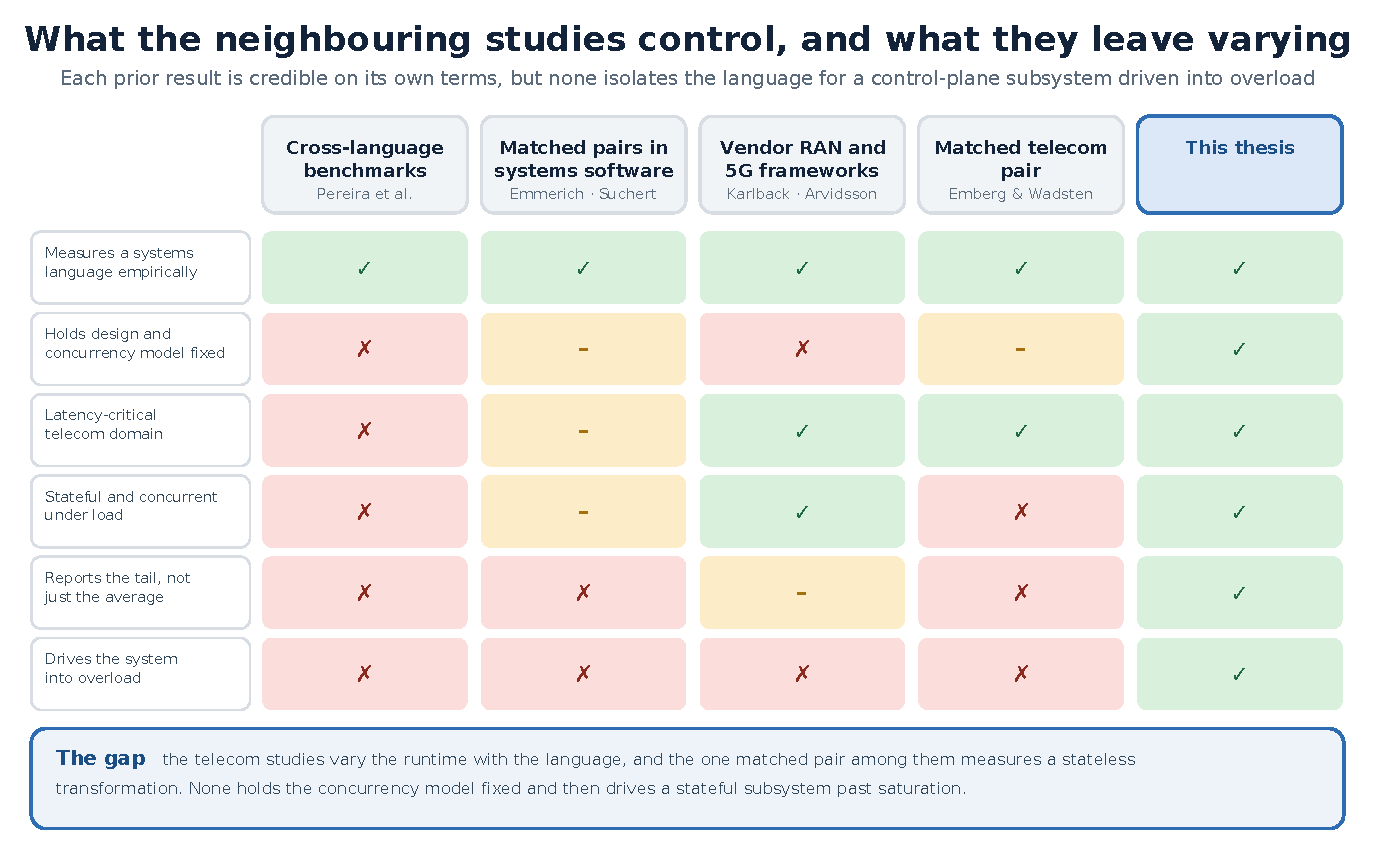
\includegraphics[width=0.78\linewidth]{diagrams/pdf/29_research_gap.pdf}
\caption[Điều các nghiên cứu lân cận kiểm soát và để thay đổi]{Điều các nghiên cứu lân cận kiểm soát và để thay đổi. Mỗi hàng là thuộc tính mà câu
trả lời có kiểm soát cho câu hỏi nghiên cứu cần. Mỗi cột là một nghiên cứu. Các so sánh chéo
ngôn ngữ đo đúng loại đối tượng nhưng sai chế độ, báo cáo trung bình trên khối lượng đa mục
đích. Cặp khớp trong phần mềm hệ thống giữ thiết kế cố định, nhưng ngoài miền này và dưới bão
hoà. Các nghiên cứu framework RAN và 5G của nhà cung cấp chạm đúng miền, và một trong số đó báo
cáo đuôi, nhưng trong tất cả ngôn ngữ thay đổi cùng runtime và mô hình tương tranh. Cặp viễn
thông khớp duy nhất, Emberg và Wadsten, kiểm soát thiết kế nhưng đo biến đổi không trạng thái.
Giữ thiết kế và mô hình tương tranh cố định cho phân hệ có trạng thái, tương tranh rồi đẩy qua
bão hoà là điều luận văn này thêm vào. Đóng góp là kiểm soát, không phải kỹ thuật đo mới.\label{fig:gapmap}}
\end{figure}

Vì vậy điều còn thiếu trong tài liệu là bằng chứng \emph{trực tiếp, có kiểm soát} cho phân hệ
mặt điều khiển đại diện: liệu Rust có thực sự giữ độ trễ đuôi và khả năng dự đoán khi quá tải
so với C++ hiện đại \emph{khi mô hình tương tranh, thuật toán và cấu trúc dữ liệu được giữ
cố định}, chính xác lớp lỗi nào nó loại bỏ và giai đoạn nào phần còn lại bị bắt, mô hình an toàn
tốn bao nhiêu về thông lượng và tài nguyên, và áp dụng tăng dần tốn bao nhiêu trong thực tế.
Lấp khoảng trống này là mục đích của bốn câu hỏi nghiên cứu. Chương tiếp theo neo chúng vào
phân hệ cụ thể, lớp lỗi và thuộc tính thời gian liên quan, và
Chương~\ref{chapter:methodology} nêu phương pháp luận để theo đuổi chúng.
